%----------------------------------------------------------------------------
%Type of document
\documentclass{beamer}

%----------------------------------------------------------------------------
%Packages
\usepackage{amsmath}
\usepackage{hyperref}
\usepackage{subfigure}
\usepackage{graphicx}

%----------------------------------------------------------------------------
%Local adjustments of settings and definitions
\setcounter{MaxMatrixCols}{10}
\setbeamertemplate{caption}[numbered]
\definecolor{links}{HTML}{2A1B81}
\hypersetup{colorlinks,linkcolor=,urlcolor=links}

%----------------------------------------------------------------------------
%Beamer theme (Madrid and Frankfurt are good options)
\usetheme{Madrid}

%----------------------------------------------------------------------------
%Start document
\begin{document}

%----------------------------------------------------------------------------
%Front matter
\title[New Keynesian Model]{The Basic New Keynesian Model}
\author[Bidder]{Rhys Bidder}
\institute[FRBSF]{Federal Reserve Bank of San Francisco}
\date{Michaelmas Term 2019}
\maketitle

%----------------------------------------------------------------------------
%Main body

\begin{frame}{Disclaimer}

The views expressed in this presentation, and all errors and omissions, should be regarded as those solely of the authors, and are not necessarily those of the Federal Reserve Bank of San Francisco, the Federal Reserve Board of Governors or the Federal Reserve System.

\end{frame}

%-------------------------------------------------------

%-------------------------------------------------------
	
\begin{frame}{The Basic New Keynesian Model}

The New Keynesian model shares many common features with the classical model but\ldots
\begin{enumerate}
\item	The classical model had fully competitive firms, whereas the NK model has monopolistically competitive firms
	\begin{itemize}
	\item	Firms have pricing power
	\item	Face a downward sloping demand curve
	\end{itemize}
\item	There are no nominal rigidities in the classical model, whereas the NK model features price stickiness
	\begin{itemize}
	\item	Various ways to model this
	\item	Common assumption: A fraction of firms are randomly `allowed' to change prices in each period
	\end{itemize}
\item	(Less important) Households buy multiple consumption goods
	\begin{itemize}
	\item	Household consumes a bundle of different consumption goods
	\item	Imperfect willingness to substitute between these goods is the source of firms' market power
	\end{itemize}
\end{enumerate}

\end{frame}

%-------------------------------------------------------

%-------------------------------------------------------
	
\begin{frame}{The Basic New Keynesian Model}

These features go hand in hand
\begin{itemize}
\item	Consider fully competitive model
\item	Suppose a firm cannot change its price
\item	If the market clearing price declines below that firm's price they would lose all demand
\end{itemize}

\vspace{2mm}
Pricing power justifies sticky prices and the decision of what price to set when firms can adjust
\begin{itemize}
\item	The (minor) adjustment to household preferences underpins the pricing power
\item	Note that there are alternative ways of motivating the pricing power
\end{itemize}

\end{frame}

%-------------------------------------------------------
\section{Households}
%-------------------------------------------------------

\begin{frame}

\begin{center}
{\LARGE Households}
\end{center}

\end{frame}

%-------------------------------------------------------

%-------------------------------------------------------
	
\begin{frame}{Households - Preferences}

Objective function of a household
\begin{equation*}
E_{0} \left[ \sum\limits_{t=0}^{\infty} \beta^{t} U \left( C_{t}, N_{t}; Z_{t} \right) \right]
\end{equation*}

Looks same as before but now $C_{t}$ is a bundle of different goods
\begin{equation}
C_{t} \equiv \left( \int_{0}^{1} C_{t}\left( i \right)^{\frac{\varepsilon-1}{\varepsilon}} di \right)^{\frac{\varepsilon}{\varepsilon-1}} \label{eqn:ds_aggregator}
\end{equation}

Sometimes this is referred to as a `Dixit-Stiglitz' aggregator
\begin{itemize}
\item	It aggregates (adds up) contributions from different types of goods
\item	Each good is indexed by $i\in[0,1]$
\item	$C_{t}(i)$ is a particular type of consumption
\item	$C_{t}$ is `overall' consumption
\end{itemize}

\end{frame}

%-------------------------------------------------------

%-------------------------------------------------------
	
\begin{frame}{Households - Preferences}

Objective function of a household
\begin{equation*}
E_{0} \left[ \sum\limits_{t=0}^{\infty} \beta^{t} U \left( C_{t}, N_{t}; Z_{t} \right) \right]
\end{equation*}

Looks same as before but now $C_{t}$ is a bundle of different goods
\begin{equation}
C_{t} \equiv \left( \textcolor{red}{\int_{0}^{1}} C_{t}\left( i \right)^{\frac{\varepsilon-1}{\varepsilon}} \textcolor{red}{di} \right)^{\frac{\varepsilon}{\varepsilon-1}} \label{eqn:ds_aggregator}
\end{equation}

Sometimes this is referred to as a `Dixit-Stiglitz' aggregator
\begin{itemize}
\item	It aggregates (\textcolor{red}{adds up}) contributions from different types of goods
\item	Each good is indexed by $i\in[0,1]$
\item	$C_{t}(i)$ is a particular type of consumption
\item	$C_{t}$ is `overall' consumption
\end{itemize}

\end{frame}


%-------------------------------------------------------

%-------------------------------------------------------
	
\begin{frame}{Households - Multiple goods}

The budget constraint is
\begin{equation*}
\underbrace{\int_{0}^{1} P_{t}(i) C_{t}(i)di}_{Total \, Expenditure} + \underbrace{Q_{n,t} B_{t}}_{Savings} \leq \overbrace{B_{t-1}}^{Payoff\, from\, Bonds} + \overbrace{W_{t} N_{t}}^{Earnings} + \overbrace{D_{t}}^{Dividends}
\end{equation*}
where we note that each consumption good has its own price, $P_{t}(i)$

\vspace{3mm}
At any optimum, the household must maximize $C_{t}$ for any amount spent on consumption goods
\begin{itemize}
\item	$C_{t}(i)$ chosen appropriately, given prices
\item	Optimal allocation across goods (see Gal\'i Ch. 3 appendix)\ldots
\end{itemize}
\begin{equation*}
C_{t}(i) = \left( \frac{P_{t}(i)}{P_{t}} \right)^{-\varepsilon} C_{t} \label{eqn:ds_optimal_cons}
\end{equation*}

\end{frame}

%-------------------------------------------------------

%-------------------------------------------------------
	
\begin{frame}{Households - Multiple goods}

The budget constraint is
\begin{equation*}
\underbrace{\int_{0}^{1} P_{t}(i) C_{t}(i)di}_{Total \, Expenditure} + \underbrace{Q_{n,t} B_{t}}_{Bond\,Purchases} \leq \overbrace{B_{t-1}}^{Payoff\, from\, Bonds} + \overbrace{W_{t} N_{t}}^{Earnings} + \overbrace{D_{t}}^{Dividends}
\end{equation*}
where we note that each consumption good has its own price, $P_{t}(i)$

\vspace{3mm}
At any optimum, the household must maximize $C_{t}$ for any amount spent on consumption goods
\begin{itemize}
\item	$C_{t}(i)$ chosen appropriately, given prices
\item	Optimal allocation across goods (see Gal\'i Ch. 3 appendix)\ldots
\end{itemize}
\begin{equation*}
C_{t}(i) = \left( \frac{P_{t}(i)}{P_{t}} \right)^{-\varepsilon} C_{t} \label{eqn:ds_optimal_cons}
\end{equation*}

\end{frame}

%-------------------------------------------------------

%-------------------------------------------------------
	
\begin{frame}{Households - Multiple goods}

Optimal demand across goods
\begin{equation*}
C_{t}(i) = \left( \frac{P_{t}(i)}{P_{t}} \right)^{-\varepsilon} C_{t}
\end{equation*}

This is associated with a price index \emph{defined} as
\begin{equation*}
P_{t} \equiv \left( \int_{0}^{1} P_{t}(i)^{1-\varepsilon}di \right)^{\frac{1}{1-\varepsilon}} \label{eqn:ds_optimal_cons_pindex}
\end{equation*}

Why is this an appropriate definition of a price index?
\begin{equation*}
\int_{0}^{1} P_{t}(i) C_{t}(i) di = P_{t} C_{t} \label{eqn:pc_expenditure}
\end{equation*}

%Note that the last expression assumes optimal demand across goods

\end{frame}

%-------------------------------------------------------

%-------------------------------------------------------
	
\begin{frame}{Households - Multiple goods}

Relative to overall demand ($C_{t}$), demand for good $i$ decreases in its relative price
\[
C_{t}(i) = \left( \frac{P_{t}(i)}{P_{t}} \right)^{-\varepsilon} C_{t}
\]

\vspace{3mm}
The elasticity of demand,  $\varepsilon$, controls strength of this effect
\begin{itemize}
\item	Large $\varepsilon \Rightarrow$ large decline in demand for good $i$
\item	Looking ahead - this will affect pricing power of firms
\item	High (low) elasticity $\Rightarrow$ low (high) market power
\item	$\varepsilon \rightarrow \infty$ represents price taking / perfect competition
\end{itemize}

\end{frame}

%-------------------------------------------------------

%-------------------------------------------------------
	
\begin{frame}{Households - Multiple goods}

Equation (\ref{eqn:pc_expenditure}) means that the budget constraint can be re-written as
\begin{equation*}
P_{t} C_{t} + Q_{n,t} B_{t} \leq B_{t-1} + W_{t} N_{t} + D_{t}
\end{equation*}

Consequently, we have the same intratemporal and intertemporal optimality conditions as in the classical model

\begin{eqnarray*}
-\frac{U_{n,t}}{U_{c,t}} 	&=& \frac{W_{t}}{P_{t}} \\
Q_{t} 					&=& \beta E_{t} \left[ \frac{U_{c,t+1}}{U_{c,t}} \frac{P_{t}}{P_{t+1}} \right]
\end{eqnarray*}

\end{frame}

%-------------------------------------------------------
\section{Firms}
%-------------------------------------------------------

\begin{frame}

\begin{center}
{\LARGE Firms}
\end{center}

\end{frame}

%-------------------------------------------------------

%-------------------------------------------------------
	
\begin{frame}{Firms - Monopolistic Competition}

There is a continuum of firms indexed by $i\in[0,1]$
\begin{itemize}
\item	They each produce a different good
\item	Identical production function
\item	Common technology
\end{itemize}
\[
Y_{t} = A_{t}N_{t}(i)^{1-\alpha}
\]

\vspace{2mm}
The technology process, $a_{t}\equiv \log{A_{t}}$, follows an AR(1)
\begin{eqnarray*}
a_{t} 				&=& 					\rho_{a} a_{t-1} + \varepsilon_{t}^{a} \\
\varepsilon_{t}^{a}	&\stackrel{iid}{\sim}&	N\left(0,\sigma_{a}^{2}\right)
\end{eqnarray*}

\end{frame}

%-------------------------------------------------------

%-------------------------------------------------------
	
\begin{frame}{Firms - Monopolistic Competition}

\[
C_{t}(i) = \left( \frac{P_{t}(i)}{P_{t}} \right)^{-\varepsilon} C_{t}
\]

Implies a demand curve for firm $i$'s good, given $C_{t}$ and $P_{t}$
\begin{itemize}
\item	Note: \textbf{Aggregate} price level and consumption are taken as given
\item	Firm can choose \textbf{its} price and (thus) \textbf{its} quantity
\end{itemize}

\vspace{2mm}
The firms thus operate in a monopolistically competitive environment
\begin{itemize}
\item	`Monopolistic' - they are the only producer of their good $i$ and can set their price
\item	`Competitive' - goods partly substitutable (limits market power)
\item	Only producer of energy drink $x$ but if `too expensive' people will shift to energy drink $y$
\end{itemize}


\end{frame}

%-------------------------------------------------------

%-------------------------------------------------------
	
\begin{frame}{Firms - Monopolistic Competition}

In a `standard' monopolistically competitive situation (see hwk.)
\begin{itemize}
\item	Firm sets its price as a markup over marginal cost
\item	Given demand curve $\Rightarrow$ picking output and employment
\item	$\varepsilon \rightarrow \infty$ shows no markup in perfectly competitive limit
\end{itemize}
\begin{eqnarray*}
P_{t}(i)^{*} &=& \frac{\varepsilon}{\varepsilon-1} MC_{t} \label{ref:flex_markup} \\
MC_{t}		&=& \frac{W_{t}}{\left( 1 - \alpha \right) A_{t} N_{t}(i)^{-\alpha}}
\end{eqnarray*}

\vspace{2mm}
But in the NK model the firm may be unable to set their price as they wish\ldots

\end{frame}

%-------------------------------------------------------

%-------------------------------------------------------
	
\begin{frame}{Firms - Price Stickiness}

Each firm may only reset its price with probability $1-\theta$
\begin{itemize}
\item	See Calvo (1983) - and hwk.
\item	Same independent probability across firms in each period
\item	Independent of time since the firm last was able to reset its price
\end{itemize}

\vspace{2mm}
This means that in each period a fraction $\theta$ of firms keep prices unchanged
\begin{itemize}
\item	Continuum of firms $i \in [0,1]$
\item	Law of large numbers
\item	Toss a fair coin a billion times and fraction heads will be $\approx 0.5$, toss it $N\rightarrow\infty$ and fraction $\rightarrow 0.5$
\item	We have infinitely many (`small') firms with prob. $\theta$ - thus fraction $\theta$ keep price fixed
\end{itemize}

\vspace{2mm}
Average duration of a given price = $\frac{1}{1-\theta}$
\begin{itemize}
\item	Natural to interpret $\theta$ as an index of price rigidity or `stickiness'
\end{itemize}

\end{frame}

%-------------------------------------------------------

%-------------------------------------------------------
	
\begin{frame}{Firms - Price Stickiness}

In every period  the distribution of prices across firms is a mixture of
\begin{enumerate}
\item	The price of the $1-\theta$ of firms who get to reoptimize
	\begin{itemize}
	\item	All set the same price since they face the same optimization problem
	\end{itemize}
\item	The prices of the $\theta$ fraction of firms whose prices were reoptimized before $t$ but are now fixed
	\begin{itemize}
	\item	Among these prices, a fraction $1-\theta$ were reoptimized in $t-1$ and a fraction $\theta$ were reoptimized before $t-1$
	\item	Among those prices reoptimized before $t-1$, a fraction $1-\theta$ were reoptimized in $t-2$ and a fraction $\theta$ were reoptimized before $t-2$
	\item	Continue the logic\ldots
	\end{itemize}
\end{enumerate}

\end{frame}

%-------------------------------------------------------

%-------------------------------------------------------
	
\begin{frame}{Firms - Optimal Pricing}

In $t$ we have prices prevailing that were reoptimized in the current period \emph{and all previous periods}
\begin{itemize}
\item	The fraction of prices in $t$ that were set in $t-j$ is declining (to zero) as $j\rightarrow \infty$
\end{itemize} 

\vspace{2mm}
When firms set their prices they do so acknowledging that\ldots
\begin{itemize}
\item	There is a distribution of prevailing prices now and in the future
%\item	Different goods but since same elasticity between all, they are all treated the same in terms of determining the optimal price for the firm, because they all have the same implication for his demand curve
\item	Their own price will prevail for a random length of time into the future
\end{itemize}

\vspace{2mm}
The problem is thus very different from standard `static' monopolistic competition that implied
\[
P_{t}(i)^{\ast} = \frac{\varepsilon}{\varepsilon-1} MC_{t}
\]

\end{frame}

%-------------------------------------------------------

%-------------------------------------------------------
	
\begin{frame}{Firms - Optimal Pricing}

Since a firm's price will prevail (with some probability) for several periods after it is set, the firms must consider the implications of that price for \emph{future} profits in those contingencies
\begin{equation*}
\max_{P_{t}^{\ast}} \sum\limits_{k=0}^{\infty} \theta^{k} E_{t} \left[ \Lambda_{t,t+k} \frac{1}{P_{t+k}} \left( P_{t}^{\ast} Y_{t+k|t} - W_{t+k}N_{t+k|t} \right) \right]
\end{equation*}

This looks (and is quite) complicated but we will go through it carefully and see that it is very intuitive after all\ldots

\end{frame}

%-------------------------------------------------------

%-------------------------------------------------------
	
\begin{frame}{Firms - Optimal Pricing}

Contribution to the value of a firm, in $t$, of profits \emph{in periods and contingencies in which $P_{t}^{\ast}$ prevails:}
\begin{equation*}
\max_{P_{t}^{\ast}} \sum\limits_{k=0}^{\infty} \theta^{k} E_{t} \left[ \Lambda_{t,t+k} \frac{1}{P_{t+k}} \left( P_{t}^{\ast} Y_{t+k|t} - W_{t+k}N_{t+k|t} \right) \right]
\end{equation*}
	
\begin{itemize}
\item	$\theta_{k}$ is the probability of $P_{t}^{\ast}$ still prevailing $k$ periods from t
\item	$\Lambda_{t,t+k}$ values the stream of real profits
	\begin{itemize}
	\item	$k$-step household SDF because households are the shareholders
	\end{itemize}
\item	$Y_{t+k|t}$ and $N_{t+k|t}$ are the output and associated employment in $t+k$ for firms who last reset their price in $t$
\item	$ P_{t}^{\ast} Y_{t+k|t} - W_{t+k}N_{t+k|t}$ are nominal profits
\item	Dividing by $P_{t+k}$ converts nominal profits to real
\end{itemize}

%\vspace{2mm}
%Note that profits from periods/contingencies in which $P_{t}^{\ast}$ has been superseded are not relevant for the choice of $P_{t}^{\ast}$

\end{frame}

%-------------------------------------------------------

%-------------------------------------------------------
	
\begin{frame}{Firms - Optimal Pricing}

Useful to clarify components of the maximand
\begin{eqnarray*}
W(P_{t}^{\ast}) &\equiv& \sum\limits_{k=0}^{\infty} \theta^{k} E_{t} \left[ \Lambda_{t,t+k} \frac{1}{P_{t+k}}  \left( \mathcal{R}(Y_{t+k|t},P_{t}^{\ast}) - \mathcal{C}(Y_{t+k|t}) \right) \right] \\
\mathcal{R}(Y_{t+k|t},P_{t}^{\ast}) &\equiv& P_{t}^{\ast} Y_{t+k|t} \qquad \quad \;\, (Revenue)\\
\mathcal{C}(Y_{t+k|t}) &\equiv& W_{t+k} \mathcal{N}(Y_{t+k|t}) \;\; (Cost)
\end{eqnarray*}
where (using the production function) we define the employment level induced by $Y_{t+k|t}$ as
\[
\mathcal{N}(Y_{t+k|t}) \equiv \left( \frac{Y_{t+k|t}}{A_{t+k}} \right)^{\frac{1}{1-\alpha}}
\]
Note: We only consider revenue and cost in the contingencies in which the price set in $t$ is still prevailing
\begin{itemize}
\item	Recall assumption: firms produce whatever is demanded at the prevailing price
\end{itemize}
	
\end{frame}

%-------------------------------------------------------

%-------------------------------------------------------
	
\begin{frame}{Firms - Optimal Pricing}

Using the demand curve implied by optimal allocation across goods
\[
Y_{t+k|t} = \left( \frac{P_{t}^{\ast}}{P_{t+k}} \right)^{-\varepsilon} C_{t+k}
\]

It is useful to define nominal marginal cost
\[
\Psi_{t+k|t} \equiv \frac{d \mathcal{C}(Y_{t+k|t})}{dY_{t+k|t}}
\]

%And, for clarity
%\[
%\xi_{t+k|t}\equiv \frac{d Y_{t+k|t}}{dP_{t}^{\ast}}
%\]
	
\end{frame}

%-------------------------------------------------------

%-------------------------------------------------------
	
\begin{frame}{Firms - Optimal Pricing}

As stated in Gal\'i (p. 56) the FOC for the choice of $P_{t}^{\ast}$ can be rearranged to be
\begin{equation}
\sum\limits_{k=0}^{\infty} \theta^{k} E_{t} \left[ \Lambda_{t,t+k} Y_{t+k|t} \frac{1}{P_{t+k}} \left( P_{t}^{\ast} - \mathcal{M} \Psi_{t+k|t}  \right) \right] = 0 \label{eqn:opt_price_cond}
\end{equation}
%or in real terms (with superscript $r$ meaning divided by $P_{t+k}$)
% \[
%\sum\limits_{k=0}^{\infty} \theta^{k} E_{t} \left[ \Lambda_{t,t+k} Y_{t+k|t} \left( P_{t}^{r,\ast} - \mathcal{M} \Psi^{r}_{t+k|t}  \right) \right] = 0
%\]

\vspace{3mm}
If $\theta=0$ then we are back in the static monopolistic competitive case
\begin{itemize}
\item	Convention is $0^{0}\equiv1$
\item	Recover static optimal markup of $P_{t}^{\ast}=\mathcal{M}  \Psi_{t}$
\item	Call $\mathcal{M}$ the `desired' or `natural' or `flex-price' markup
\end{itemize}
	
\end{frame}

%-------------------------------------------------------

%-------------------------------------------------------
	
\begin{frame}{Firms - Optimal Pricing}

If $\theta \in (0,1)$ then the static condition will (generically) not hold
\[
P_{t}^{\ast}\neq\mathcal{M}  \Psi_{t}
\]

However, firms are setting prices to try to keep the deviations from this condition `small' in all periods
\begin{itemize}
\item	The optimality condition is a weighted sum of deviations of the firm's price in $t+k$ from $\mathcal{M}  \Psi_{t+k|t}$
\item	Intuition for weights\ldots
	\begin{itemize}
	\item	$\theta^{k}\Rightarrow$ particularly care about near future
	\item	$\Lambda_{t,t+k}\Rightarrow$ particularly care about reduced profits when MU is high
	\item	$Y_{t+k|t}\Rightarrow$ static suboptimality more concerning if producing a lot
	\end{itemize}
\end{itemize}

\end{frame}

%%-------------------------------------------------------
%
%%-------------------------------------------------------
%	
%\begin{frame}{Firms - Optimal Pricing}
%
%In a nonstochastic (without randomness) version of the model with zero inflation\ldots
%\begin{itemize}
%\item	All firms' prices, outputs and marginal costs are identical
%\item	$\Lambda_{t,t+k}=\beta^{k}$
%\item	$P_{t}=P_{t+k}$
%\item	$Y_{t+k|t}=Y$
%\item	$\Psi^{r}_{t+k|t}=\Psi^{r}$
%\item	$\Psi_{t+k|t}=\Psi_{t}$
%\end{itemize}
%
%\vspace{2mm}
%Given this, the optimal price setting condition shows that
%\[
%P_{t}=\mathcal{M} \Psi_{t}
%\]
%
%Subscript $t$ simply reflects that inflation is zero but aggregate price \textbf{level} not pinned down in SS (why is this unimportant?)
%
%\end{frame}

%-------------------------------------------------------

%-------------------------------------------------------
	
\begin{frame}{Firms - Optimal Pricing}

Approximating around the zero inflation steady state we obtain (lower case means logs)
\begin{eqnarray}
p_{t}^{\ast} &=& 	\mu + (1-\beta \theta) \sum\limits_{k=0}^{\infty} (\beta \theta)^{k} E_{t}\left[ \psi_{t+k|t} \right] \\
\mu 		&\equiv& \log{\mathcal{M}} \nonumber
\end{eqnarray}

\begin{itemize}
\item	Firms markup by $\mathcal{M}$ but not over current marginal cost
\item	Instead they markup over a weighted average of current and future marginal costs
\item	Weights $\propto$ time discount ($\beta^{k}$) and probability of price prevailing ($\theta^{k}$)
\end{itemize}

\vspace{2mm}
Thus, firms set prices in a \textbf{forward looking} manner

\end{frame}

%%-------------------------------------------------------
%
%%-------------------------------------------------------
%	
%\begin{frame}{Firms - Aggregate Price Dynamics}
%
%Recall the definition of the price index, $P_{t}$ implies
%\[
%P_{t}^{1-\varepsilon} = \int\limits_{0}^{1} P_{t}(i)^{1-\varepsilon} di
%\]
%
%A fraction of $1-\theta$ firms reset to $P_{t}^{\ast}$ and the rest keep their previous price
%\begin{eqnarray}
%P_{t}^{1-\varepsilon} &=& \int\limits_{0}^{\theta} P_{t}(i)^{1-\varepsilon} di + \int\limits_{\theta}^{1} P_{t}(i)^{1-\varepsilon} di \nonumber \\
%&=& \int\limits_{0}^{\theta} P_{t}(i)^{1-\varepsilon} di + (1-\theta) (P_{t}^{\ast})^{1-\varepsilon} di \label{eqn:price_evol}
%\end{eqnarray}
%where WLOG we reordered firms so the first $\theta$ fraction of the unit interval are the `fixed' firms
%
%\end{frame}
%
%%-------------------------------------------------------
%
%%-------------------------------------------------------
%	
%\begin{frame}{Firms - Aggregate Price Dynamics}
%
%Consider the first term on the LHS of equation (\ref{eqn:price_evol})
%\[
%\int\limits_{0}^{\theta} P_{t}(i)^{1-\varepsilon} di
%\]
%
%This is effectively like calculating the price index for $t-1$ but over a `smaller' set of firms
%\begin{itemize}
%\item	The firms keeping prices fixed were chosen completely at random
%\item	$\Rightarrow$ the pattern of prices among them is the same as the \emph{overall} pattern in $t-1$
%\item	$\Rightarrow$ `average' price the same but they make only a $\theta$ contribution to the price level in $t$
%\end{itemize}
%
%\end{frame}
%
%%-------------------------------------------------------
%
%%-------------------------------------------------------
%	
%\begin{frame}{Firms - Aggregate Price Dynamics}
%
%Given the preceding logic, we have
%\begin{eqnarray*}
%P_{t}^{1-\varepsilon} &=& \int\limits_{0}^{\theta} P_{t}(i)^{1-\varepsilon} di + (1-\theta) (P_{t}^{\ast})^{1-\varepsilon} di \\
%&=&\theta P_{t-1}^{1-\varepsilon} + (1-\theta) (P_{t}^{\ast})^{1-\varepsilon} di
%\end{eqnarray*}
%
%And dividing by $P_{t-1}^{1-\varepsilon}$ we obtain
%\begin{equation}
%\Pi_{t}^{1-\varepsilon} = \theta + (1-\theta)\left( \frac{P_{t}^{\ast}}{P_{t-1}} \right)^{1-\varepsilon} \label{eqn:gross_infl}
%\end{equation}
%where, recall,  $\Pi_{t}\equiv P_{t}/P_{t-1}$ is the gross inflation rate
%
%\end{frame}

%-------------------------------------------------------

%-------------------------------------------------------
	
\begin{frame}{Firms - Aggregate Price Dynamics}

As shown in the text\ldots
\begin{equation*}
\Pi_{t}^{1-\varepsilon} = \theta + (1-\theta)\left( \frac{P_{t}^{\ast}}{P_{t-1}} \right)^{1-\varepsilon} \label{eqn:gross_infl}
\end{equation*}
where, recall,  $\Pi_{t}\equiv P_{t}/P_{t-1}$ is the gross inflation rate

\vspace{3mm}
%If we take a log-linear approximation of equation (\ref{eqn:gross_infl}) and rearrange we obtain
If we take a log-linear approximation and rearrange we obtain
\[
p_{t} = \theta p_{t-1} + (1-\theta) p_{t}^{\ast}
\]

\vspace{3mm}
Thus the current price level is a weighted average of last period's price level and the new reset price
\begin{itemize}
\item	Price level evolves as $p_{t}^{\ast}$ typically $\neq p_{t-1}$
\item	Weights are intuitively connected to $\theta$
\end{itemize}

\end{frame}

%-------------------------------------------------------
\section{Equilibrium - Non-policy Block}
%-------------------------------------------------------

\begin{frame}

\begin{center}
{\LARGE Equilibrium - Non-policy Block}
\end{center}

\end{frame}

%-------------------------------------------------------

%-------------------------------------------------------
	
\begin{frame}[label=jumpback]{Equilibrium - Non-policy bloc}

Household optimality conditions
\begin{itemize}
\item	Labor supply
\item	Intertemporal optimality and the definition of the SDF
\item	Optimal allocation of consumption across goods (implies demand curves for firms)
\item	SDF will be used by firm (owned by households)
\end{itemize}

\vspace{2mm}
Firm optimality conditions
\begin{itemize}
\item	Optimal price setting
\item	Labor demand and supply of good $i$ are implied by the price decision
	\begin{itemize}
	\item	Production function taken as given
	\item	Assume firms supply what is demanded at a given price
	\end{itemize}
\end{itemize}

\vspace{2mm}
We use these and market clearing/feasibility assumptions to solve for equilibrium (we will also need a monetary policy block)
\hyperlink{jump}{\beamergotobutton{Extra derivations}}

\end{frame}

%-------------------------------------------------------

%-------------------------------------------------------
	
\begin{frame}{Equilibrium - Non-policy bloc}

Recall (from previous lectures) that firm marginal cost is wage over marginal product of labor (need 1/MPL for marginal unit of output, and pay that unit $W$):
\[
\psi_{t}(i) = w_{t} - \left( a_{t} - \alpha n_{t}(i) + \log{(1-\alpha)} \right)
\]

Then, using the approximation $n_{t}=\int\limits_{0}^{1} n_{t}(i)di$, we can show
\[
\psi_{t+k|t} = \psi_{t+k} + \alpha (n_{t+k|t} - n_{t+k})
\]

If $\alpha>0$, firms who haven't reset since $t$ have MC higher than the average if their employment levels are relatively high (except for $\alpha=0$ - why?)
\begin{itemize}
\item	$\Leftrightarrow$ their output is relatively high (why? use the prod. fn.)
\item	$\Leftrightarrow$ their price is relatively low (why? use the dem. curve)
\end{itemize}

\[
\psi_{t+k|t} = \psi_{t+k} - \frac{\alpha \varepsilon}{1-\alpha} (p_{t}^{\ast} - p_{t+k})
\]


\end{frame}

%-------------------------------------------------------

%-------------------------------------------------------
	
\begin{frame}{Equilibrium - Non-policy bloc}

We derived an expression for $p_{t}^{\ast}$ earlier in terms of expected $\psi_{t+k|t}$ - combining that with the expression for $\psi_{t+k|t}$\ldots 
\[
\pi_{t} 			=	\beta E_{t}[ \pi_{t+1} ]	 -\lambda \hat{\mu}_{t}
\]
with
\begin{eqnarray*}
\lambda 			&\equiv& 	\theta^{-1}(1-\theta)(1-\beta\theta)\Theta > 0\\
\Theta 			&\equiv& 	\frac{1-\alpha}{1-\alpha + \alpha \varepsilon}
\end{eqnarray*}
and where
\begin{eqnarray*}
\mu_{t} 		&\equiv&	 p_{t} - \psi_{t} \qquad \!\!Markup\;over\;marginal\;cost\\
\hat{\mu}_{t} 	&\equiv&	 \mu_{t} - \mu \qquad Deviation\;from\;desired\;markup
\end{eqnarray*}

\end{frame}

%-------------------------------------------------------

%-------------------------------------------------------
	
\begin{frame}{Equilibrium - Non-policy bloc}

Inflation reflects expected path of markup `gaps'
\[
\pi_{t} = -\lambda \sum\limits_{k=0}^{\infty} \beta^{k} E_{t}[\hat{\mu}_{t+k}]
\]

\begin{itemize}
\item	Markups expected to be below desired $\Rightarrow \pi_{t}>0$
\item	Markups expected to be at desired level $\Rightarrow \pi_{t}=0$
\item	Markups expected to be above desired level $\Rightarrow \pi_{t}<0$
\end{itemize}

\vspace{3mm}
$\Rightarrow$ pricing decisions of reoptimizing firms tends to restore the desired markup and \textbf{these adjustments induce non-zero inflation}

\end{frame}

%%-------------------------------------------------------
%
%%-------------------------------------------------------
%	
%\begin{frame}{Equilibrium - Non-policy bloc}
%
%Expressed more intuitively perhaps\ldots
%\[
%\pi_{t} = \lambda \sum\limits_{k=0}^{\infty} \beta^{k} E_{t}[\hat{mc}_{t+k}]
%\]
%where $\hat{mc_{t}}$ is the deviation of real marginal cost from desired
%
%\begin{itemize}
%\item	Marginal cost expected to be below desired $\Rightarrow \pi_{t}<0$
%\item	Marginal cost expected to be at desired level $\Rightarrow \pi_{t}=0$
%\item	Marginal cost expected to be above desired level $\Rightarrow \pi_{t}>0$
%\end{itemize}
%
%\vspace{3mm}
%$\Rightarrow$ pricing decisions of reoptimizing firms tends to restore the desired marginal cost $\Leftrightarrow$ desired scale of operations
%
%\end{frame}

%-------------------------------------------------------

%-------------------------------------------------------
	
\begin{frame}{Equilibrium - Non-policy bloc}

We want to connect the markup to the level of activity ($y_{t}$) in the economy
\begin{itemize}
\item	Note that $\mu_{t}=-mc_{t}$ where $mc_{t}$ is \textbf{real} marginal cost
\item	Use this to derive an expression for $\mu_{t}$ in terms of $y_{t}$ and $a_{t}$
\end{itemize}
\begin{eqnarray*}
\mu_{t} &=& p_{t} - \psi_{t}	\\
		&=& -(w_{t} - p_{t}) + (a_{t} - \alpha n_{t} + \log{(1-\alpha)}) \\
		&=& -(\sigma y_{t} + \varphi n_{t}) + (a_{t} - \alpha n_{t} + \log{(1-\alpha)}) \\
		&=& - \left( \sigma + \frac{\varphi + \alpha}{1-\alpha} \right)y_{t} + \left( \frac{1+\varphi}{1-\alpha} \right) a_{t} + \log{(1-\alpha)}
\end{eqnarray*}

%\begin{itemize}
%\item	Note that \emph{equilbrium} real marginal cost depends on `scale' ($y_{t}$) even with $\alpha=0$ (constant returns)
%\item	Why? \emph{In equilibrium} the wage rate must change - whereas an individual firm takes it as given
%\end{itemize}

\end{frame}

%-------------------------------------------------------

%-------------------------------------------------------
	
\begin{frame}{Equilibrium - Non-policy bloc}

We want to connect the markup to the level of activity ($y_{t}$) in the economy
\begin{itemize}
\item	Note that $\mu_{t}=-mc_{t}$ where $mc_{t}$ is \textbf{real} marginal cost
\item	Use this to derive an expression for $\mu_{t}$ in terms of $y_{t}$ and $a_{t}$
\end{itemize}
\begin{eqnarray*}
\mu_{t} &=& p_{t} - \psi_{t}	\\
		&\stackrel{\textcolor{red}{\psi_{t}}}=& -(\textcolor{red}{w_{t}} - p_{t}) +\textcolor{red}{ (a_{t} - \alpha n_{t} + \log{(1-\alpha)})} \\
		&\stackrel{\textcolor{red}{HHOLD}}=& -(\textcolor{red}{\sigma c_{t} + \varphi n^{S}_{t}}) + (a_{t} - \alpha n^{\textcolor{red}{D}}_{t} + \log{(1-\alpha)}) \\
		&=& - \left( \sigma + \frac{\varphi + \alpha}{1-\alpha} \right)y_{t} + \left( \frac{1+\varphi}{1-\alpha} \right)a_{t} + \log{(1-\alpha)}
\end{eqnarray*}

%\begin{itemize}
%\item	Note that \emph{equilbrium} real marginal cost depends on `scale' ($y_{t}$) even with $\alpha=0$ (constant returns)
%\item	Why? \emph{In equilibrium} the wage rate must change - whereas an individual firm takes it as given
%\end{itemize}

\end{frame}

%-------------------------------------------------------

%-------------------------------------------------------
	
\begin{frame}{Equilibrium - Non-policy bloc}

We want to connect the markup to the level of activity ($y_{t}$) in the economy
\begin{itemize}
\item	Note that $\mu_{t}=-mc_{t}$
\item	Use this to derive an expression for $\mu_{t}$ in terms of $y_{t}$ and $a_{t}$
\end{itemize}
\begin{eqnarray*}
\mu_{t} &=& p_{t} - \psi_{t}	\\
		&=& -(w_{t} - p_{t}) + (a_{t} - \alpha n_{t} + \log{(1-\alpha)}) \\
		&=& -(\sigma y_{t} + \varphi n_{t}) + (a_{t} - \alpha n_{t} + \log{(1-\alpha)}) \\
		&=& - \left( \sigma + \frac{\varphi + \alpha}{1-\alpha} \right)y_{t} + \left( \frac{1+\varphi}{1-\alpha} \right)a_{t}+ \log{(1-\alpha)}
\end{eqnarray*}

%\begin{itemize}
%\item	Note that \emph{equilbrium} real marginal cost depends on `scale' ($y_{t}$) even with $\alpha=0$ (constant returns)
%\item	Why? \emph{In equilibrium} the wage rate must change - whereas an individual firm takes it as given
%\end{itemize}

\end{frame}

%-------------------------------------------------------

%-------------------------------------------------------
	
\begin{frame}{Equilibrium - Non-policy bloc}

A \textbf{very important concept} to grasp is the `natural' value of a (real) variable
\begin{itemize}
\item	It is the value that prevails in the `flexible price' form of this model
\item	We obtain this by setting $\theta=0$
	\begin{itemize}
	\item	There is no price stickiness
	\item	All firms can reset price in each period
	\item	Markups are always $=$ desired ($P_{t}=\mathcal{M}\Psi_{t}$)
	\item	Firms are always operating at desired scale
	\end{itemize}
\end{itemize}

\vspace{2mm}
Not equivalent to the `steady state'
\begin{itemize}
\item	Fluctuations in technology will shift the natural rate over time
\item	\textbf{It isn't constant}
\end{itemize}

\end{frame}

%-------------------------------------------------------

%-------------------------------------------------------
	
\begin{frame}{Equilibrium - Non-policy bloc}

Since $\theta=0$ is just a special case of the economy we have been discussing, all our equations still apply
\[
\textcolor{red}{\mu_{t}} = - \left( \sigma + \frac{\varphi + \alpha}{1-\alpha} \right)\textcolor{red}{y_{t}} + \left( \frac{1+\varphi}{1-\alpha} \right)a_{t}+ \log{(1-\alpha)}
\]

Thus by imposing that the markup is constantly at the desired level, we can \emph{define} the natural rate of output
\begin{eqnarray}
y^{n}_{t} 	&=& 		\psi_{y} + \psi_{y,a} a_{t} \nonumber \\
\psi_{y} 	&\equiv& 	-\frac{(1-\alpha)(\mu-\log{(1-\alpha)})}{\sigma(1-\alpha)+\varphi+\alpha} \nonumber \\
\psi_{y,a}	&\equiv& 	\frac{1+\varphi}{\sigma(1-\alpha) + \varphi + \alpha} \nonumber
\end{eqnarray}

\end{frame}

%-------------------------------------------------------

%-------------------------------------------------------
	
\begin{frame}{Equilibrium - Non-policy bloc}

Since $\theta=0$ is just a special case of the economy we have been discussing, all our equations still apply
\[
\textcolor{red}{\mu} = - \left( \sigma + \frac{\varphi + \alpha}{1-\alpha} \right)\textcolor{red}{y^{n}_{t}} + \left( \frac{1+\varphi}{1-\alpha} \right)a_{t}+ \log{(1-\alpha)}
\]

Thus by imposing that the markup is constantly at the desired level, we can \emph{define} the natural rate of output
\begin{eqnarray*}
y^{n}_{t} 	&=& 		\psi_{y} + \psi_{y,a} a_{t} \\
\psi_{y} 	&\equiv& 	-\frac{(1-\alpha)(\mu-\log{(1-\alpha)})}{\sigma(1-\alpha)+\varphi+\alpha} \\
\psi_{y,a}	&\equiv& 	\frac{1+\varphi}{\sigma(1-\alpha) + \varphi + \alpha}
\end{eqnarray*}

\end{frame}

%-------------------------------------------------------

%-------------------------------------------------------
	
\begin{frame}{Equilibrium - Non-policy bloc}

Since $\theta=0$ is just a special case of the economy we have been discussing, all our equations still apply
\[
\mu = - \left( \sigma + \frac{\varphi + \alpha}{1-\alpha} \right)y^{n}_{t} + \left( \frac{1+\varphi}{1-\alpha} \right)a_{t}+ \log{(1-\alpha)}
\]

Thus by imposing that the markup is constantly at the desired level, we can \emph{define} the natural rate of output
\begin{eqnarray}
y^{n}_{t} 	&=& 		\psi_{yn} + \psi_{yn,a} a_{t} \nonumber \\
\psi_{yn} 	&\equiv& 	-\frac{(1-\alpha)(\mu-\log{(1-\alpha)})}{\sigma(1-\alpha)+\varphi+\alpha} \nonumber \\
\psi_{yn,a}	&\equiv& 	\frac{1+\varphi}{\sigma(1-\alpha) + \varphi + \alpha} \nonumber
\end{eqnarray}

\end{frame}

%-------------------------------------------------------

%-------------------------------------------------------
	
\begin{frame}{Equilibrium - Non-policy bloc}

Compare natural rate of output\ldots
\begin{eqnarray*}
y^{n}_{t} 	&=& 		\psi_{yn} + \psi_{yn,a} a_{t} \\
\textcolor{red}{\psi_{yn}} 	&\equiv& 	-\frac{(1-\alpha)(\textcolor{red}{\mu}-\log{(1-\alpha)})}{\sigma(1-\alpha)+\varphi+\alpha} \\
\psi_{ny,a}	&\equiv& 	\frac{1+\varphi}{\sigma(1-\alpha) + \varphi + \alpha}
\end{eqnarray*}

\ldots with output in Classical model (see lecture 2)
\begin{eqnarray*}
y^{c}_{t} 		&=& 		\psi_{yc} + \psi_{yc,a} a_{t} \\
\psi_{yc} 		&\equiv& 	\frac{(1-\alpha)\log{(1-\alpha)}}{\sigma(1-\alpha)+\varphi+\alpha} \\
\psi_{yc,a}		&\equiv& 	\frac{1+\varphi}{\sigma(1-\alpha) + \varphi + \alpha}
\end{eqnarray*}

\end{frame}

%-------------------------------------------------------

%-------------------------------------------------------
	
%\begin{frame}{Equilibrium - Non-policy bloc}
%
%\begin{itemize}
%\item	Recall $\exp{(\mu)} \equiv \mathcal{M} \equiv \frac{\varepsilon}{\varepsilon - 1}$
%	\begin{itemize}
%	\item	As $\varepsilon\rightarrow\infty$ we get perfect competition (price taking) and zero markup
%	\end{itemize}
%\vspace{2mm}
%\item	Monopolistic competition $\Rightarrow$ less output than perfect competition
%	\begin{itemize}
%	\item	Firms face a downward sloping demand curve
%	\item	Must reduce price to sell more
%	\item	But lower price will apply to \emph{all} units they sell (not just marginal)
%	\item	So not profit maximizing
%	\end{itemize}
%\vspace{2mm}
%\item	Gains from trade `left on the table'
%	\begin{itemize}
%	\item	Markup $\Rightarrow$ wedge between MB to consumer and the MC to firm
%	\item	Consumer would willingly compensate firm for marginal unit
%	\item	$\Rightarrow$ deadweight loss
%	\end{itemize}
%\end{itemize}
%
%\vspace{2mm}
%NOTE: This issue is covered in homework 2 (in a simpler context)
%
%\end{frame}

%-------------------------------------------------------

%-------------------------------------------------------
	
\begin{frame}{Equilibrium - Non-policy bloc}

Monopolistic competition even suppresses output \textbf{in steady state}
\begin{itemize}
\item	To see this, put $a_{t}$ to its steady state / unconditional mean of zero
\end{itemize}

\vspace{3mm}
This means that even eliminating price stickiness won't get us back to the (efficient) Classical model
\begin{itemize}
\item	Emphasizes that NK model differs in price stickiness \textbf{and} in having competitive distortions
\end{itemize}

\vspace{3mm}
See homeworks for extensive discussion of monopolistic competition and Pigouvian subsidy

\end{frame}

%-------------------------------------------------------

%-------------------------------------------------------
	
\begin{frame}{Equilibrium - Non-policy bloc}

Returning to the expression for the natural rate of output\ldots
\[
y^{n}_{t} 	= 		\psi_{yn} + \psi_{yn,a} a_{t}
\]
The natural rate of output \textbf{does not depend on}
\begin{itemize}
\item $z_{t}$
\item Monetary policy
\end{itemize}

\vspace{3mm}
Gaps between natural and actual versions of variables reflect price stickiness
\begin{itemize}
\item	We will see price stickiness implies real effects of monetary policy
\item	Monetary policy can influence these gaps
\end{itemize}

\end{frame}

%-------------------------------------------------------

%-------------------------------------------------------
	
\begin{frame}{Equilibrium - Non-policy bloc}

We define the `\emph{output gap}'
\[
\tilde{y}_{t}\equiv y_{t}-y^{n}_{t}
\]

The phrase `output gap' is used by various people with various meanings
\begin{itemize}
\item	In the NK model it means something \emph{very} specific
\item	$y^{n}_{t}$ is a particular theoretical object and not some smooth `trend' or `moving average'
\item	$y_{t}^{n}$ emerges from an imaginary world with flexible prices and a very particular structure
\end{itemize}

\vspace{2mm}
An empirical question whether commonly used `trends' are similar to $y^{n}_{t}$
\begin{itemize}
\item	Remember, our model is only a simplification of reality
\item	Using a statistical rather than model-based gap may still be useful
\end{itemize}

\end{frame}

%-------------------------------------------------------

%-------------------------------------------------------
	
\begin{frame}{Equilibrium - Non-policy bloc}

Using (for $y_{t}$ \textbf{and} $y^{n}_{t}$)\ldots
\[
\mu_{t} = - \left( \sigma + \frac{\varphi + \alpha}{1-\alpha} \right)y_{t} + \left( \frac{1+\varphi}{1-\alpha} \right)a_{t} + \log{(1-\alpha)}
\]
combined with\ldots
\[
\pi_{t} = \beta E_{t}[\pi_{t+1}] - \lambda \hat{\mu}_{t}
\]
we obtain
\begin{equation}
\pi_{t} = \beta E_{t}[\pi_{t+1}]  + \kappa \tilde{y}_{t} \label{eqn:nkpc}
\end{equation}
where
\[
\kappa \equiv \lambda \left(  \sigma + \frac{\varphi + \alpha}{1-\alpha} \right)
\]

\end{frame}

%-------------------------------------------------------

%-------------------------------------------------------

\begin{frame}

\begin{center}
{\Huge\textcolor{red}{ $\pi_{t} = \beta E_{t}[\pi_{t+1}]  + \kappa \tilde{y}_{t}$}}
\end{center}

\end{frame}

%-------------------------------------------------------

%-------------------------------------------------------
	
\begin{frame}{Equilibrium - Non-policy bloc}

This relation is called the `New Keynesian Phillips Curve' (NKPC)
\begin{equation*}
\pi_{t} = \beta E_{t}[\pi_{t+1}]  + \kappa \tilde{y}_{t}
\end{equation*}

\begin{itemize}
\item	Phillips (1958) observed an (apparent) relationship between (wage) inflation and a measure of unemployment
\item	Investigating the relationship between (wage and/or price) inflation and activity (employment, growth, output gap \ldots) has been a central macro question since\ldots forever!
\item	For a long time a relationship was asserted (particularly by Keynesians) but with little or no theoretical foundations
\item	The New Keynesian model proposes microeconomic foundations that are internally consistent, within a General Equilibrium framework
\end{itemize}

\vspace{2mm}
May not be an ideal model - \textbf{but a huge intellectual achievement!}

\end{frame}

%-------------------------------------------------------

%-------------------------------------------------------
	
\begin{frame}{Equilibrium - Non-policy bloc}

To obtain an `Dynamic IS' relationship we use the household intertemporal optimality condition (with $y_{t}=c_{t}$ implicit)
\[
y_{t} = E_{t} \left[ y_{t+1} \right] - \frac{1}{\sigma} \left(i_{t} - E_{t}\left[ \pi_{t+1} \right] \right) + \frac{1}{\sigma} \left( \rho + \left( 1 - \rho_{z} \right) z_{t} \right)
\]

Setting $y_{t}=y^{n}_{t}$, and using our solution for $y^{n}_{t}$, we define
\begin{eqnarray}
r^{n}_{t} 	&\equiv&	-\sigma (1-\rho_{a})\psi_{y,a}a_{t} + \rho + (1-\rho_{z})z_{t} \label{eqn:rn_equilib}\\
			&\equiv&	\psi_{rn} + \psi_{rn,a} a_{t} + \psi_{rn,z} z_{t} \nonumber
\end{eqnarray}

This `natural' real interest rate would prevail in a flexible price economy and we can show
\begin{eqnarray}
\tilde{y}_{t} &=& E_{t} \left[ \tilde{y}_{t+1} \right] - \frac{1}{\sigma} \left(i_{t} - E_{t}\left[ \pi_{t+1} \right]  - r^{n}_{t} \right) \label{eqn:dyn_IS} \\
% &=& E_{t} \left[ \tilde{y}_{t+1} \right] - \frac{1}{\sigma} \left(r_{t}  - r^{n}_{t} \right) \nonumber% \\
&=& -\frac{1}{\sigma} \sum\limits_{k=0}^{\infty} E_{t}[ r_{t+k}  - r^{n}_{t+k} ] \nonumber
\end{eqnarray}

\end{frame}

%-------------------------------------------------------

%-------------------------------------------------------

\begin{frame}

\begin{center}
{\huge\textcolor{red}{ $\tilde{y}_{t} = E_{t} \left[ \tilde{y}_{t+1} \right] - \frac{1}{\sigma} \left(i_{t} - E_{t}\left[ \pi_{t+1} \right]  - r^{n}_{t} \right) $}}
\end{center}

\end{frame}

%-------------------------------------------------------

%-------------------------------------------------------
	
\begin{frame}{Equilibrium - Non-policy bloc}

At this point we have
\begin{eqnarray}
\tilde{y}_{t} &\equiv&	 y_{t} - y^{n}_{t}							\\
\pi_{t}		&=& 		\beta E_{t}[ \pi_{t+1} ] + \kappa \tilde{y}_{t}	\\
\tilde{y}_{t} &=& 		E_{t} \left[ \tilde{y}_{t+1} \right] - \frac{1}{\sigma} \left(i_{t} - E_{t}\left[ \pi_{t+1} \right]  - r^{n}_{t} \right)														\\
y^{n}_{t}	&=&		\psi_{yn} + \psi_{yn,a} a_{t}					\\
r^{n}_{t}	&=&		\psi_{rn} + \psi_{rn,a} a_{t} + \psi_{rn,z} z_{t}
\end{eqnarray}

These equations constitute the `non-policy' block of the NK model
\begin{itemize}
\item	NKPC determines inflation given an expected path for the output gap
\item	DIS determines the output gap given an expected path for the natural and actual real interest rates
\item	The real interest rate reflects expected inflation and the nominal interest rate, which is set by policy
\end{itemize}

\end{frame}

%-------------------------------------------------------

%-------------------------------------------------------
	
\begin{frame}{Equilibrium - Non-policy block}

At this point we have
\begin{eqnarray}
\tilde{y}_{t} &\equiv&	 y_{t} - y^{n}_{t}							\\
\pi_{t}		&=& 		\beta E_{t}[ \pi_{t+1} ] + \kappa \tilde{y}_{t}	\\
\tilde{y}_{t} &=& 		E_{t} \left[ \tilde{y}_{t+1} \right] - \frac{1}{\sigma} \left(\textcolor{red}{i_{t}} - E_{t}\left[ \pi_{t+1} \right]  - r^{n}_{t} \right)														\\
y^{n}_{t}	&=&		\psi_{yn} + \psi_{yn,a} a_{t}					\\
r^{n}_{t}	&=&		\psi_{rn} + \psi_{rn,a} a_{t} + \psi_{rn,z} z_{t}
\end{eqnarray}

These equations constitute the `non-policy' block of the NK model
\begin{itemize}
\item	NKPC determines inflation given an expected path for the output gap
\item	DIS determines the output gap given an expected path for the natural and actual real interest rates
\item	The real interest rate reflects expected inflation and \textcolor{red}{the nominal interest rate, which is set by policy}
\end{itemize}

\end{frame}

%-------------------------------------------------------
\section{Equilibrium - Introducing Policy}
%-------------------------------------------------------

\begin{frame}

\begin{center}
{\LARGE Equilibrium - Introducing Policy}
\end{center}

\end{frame}

%-------------------------------------------------------

%-------------------------------------------------------
	
\begin{frame}{Equilibrium - Introducing policy}

We can't solve for the real variables without specifying monetary policy
\begin{itemize}
\item	Price stickiness $\Rightarrow$ expected inflation does not move 1:1 with $i_{t}$
\item	$r_{t} = i_{t} - E_{t}[\pi_{t+1}] \Rightarrow r_{t}$ is affected by policy actions
\item	Agents' actions influenced by $r_{t}$ (intertemporal terms of trade)
\end{itemize}

\vspace{2mm}
We imagine $i_{t}$ being set according to a policy `rule'\ldots
\begin{eqnarray*}
i_{t} 		&=& \rho + \phi_{\pi} \pi_{t} + \phi_{y} \hat{y}_{t} + v_{t} \\
\hat{y}_{t}	&=& y_{t} - y	\\
v_{t} 		&=& \rho_{v} v_{t-1} + \varepsilon^{v}_{t}
\end{eqnarray*}

These sort of rules are called `Taylor Rules' (after Taylor 1993 and 1999)
\begin{itemize}
\item	Assume $\phi_{\pi}>1$ and it is standard to assume $\phi_{y}>0$
\item	$v_{t}$ is a policy `shock'
\end{itemize}

\end{frame}

%-------------------------------------------------------

%-------------------------------------------------------
	
\begin{frame}{Equilibrium - Introducing policy}

The system we must solve is
\begin{eqnarray*}
i_{t} 		&=& \rho + \phi_{\pi} \pi_{t} + \phi_{y} \hat{y}_{t} + v_{t} 		\\
			&=& \rho + \phi_{\pi} \pi_{t} + + \phi_{y} \tilde{y}_{t} + \phi_{y} \hat{y}^{n}_{t} + v_{t} 		\\
r^{n}_{t}	&=& \rho - \sigma(1-\rho_{a})\psi_{yn,a}a_{t} + (1-\rho_{z})z_{t}	\\
\tilde{y}_{t} &=& -\frac{1}{\sigma} \left( i_{t} - E_{t}[\pi_{t+1}] - r^{n}_{t}) + E_{t}[ \tilde{y}_{t+1} ] \right)
\end{eqnarray*}

The solution will be expressions for $\tilde{y}_{t}$ and $\pi_{t}$ in terms of some combination of shocks ($a_{t}$, $z_{t}$ and $v_{t}$)
\begin{itemize}
\item	Recall, we already know $r^{n}_{t}$ and $y^{n}_{t}$ in terms of shocks
\end{itemize}

\end{frame}

%-------------------------------------------------------

%-------------------------------------------------------
	
\begin{frame}{Equilibrium - Introducing policy}

Although it is natural to look for equilibrium functions
\begin{eqnarray*}
\pi_{t} 		&=& \psi_{\pi,a} a_{t} + \psi_{\pi,z} z_{t} + \psi_{\pi,v} v_{t} \\
\tilde{y}_{t} &=& \psi_{\tilde{y},a} a_{t} + \psi_{\tilde{y},z} z_{t} + \psi_{\tilde{y},v} v_{t}
\end{eqnarray*}

Gal\'i looks for expressions in terms of the `composite' shock, $u_{t}$
\begin{eqnarray*}
\pi_{t} 		&=& \psi_{\pi,u} u_{t} \\
\tilde{y}_{t} &=& \psi_{\tilde{y},u} u_{t} \\
u_{t}		&=& -\psi_{yn,a}\left( \phi_{y} + \sigma(1-\rho_{a}) \right)a_{t} + (1-\rho_{z})z_{t} - v_{t}
\end{eqnarray*}

He then makes the assumption that $u_{t}$ follows an AR(1)
\begin{itemize}
\item	Given this, he derives $\psi_{\pi,u}$ and $\psi_{\tilde{y},u}$
\item	Only correct if one shock hits at any one time
\item	It \emph{works} but it makes things unclear
\end{itemize}

\end{frame}

%-------------------------------------------------------
\section{Response to Shocks}
%-------------------------------------------------------

\begin{frame}

\begin{center}
{\LARGE Response to Shocks}
\end{center}

\end{frame}

%-------------------------------------------------------

%-------------------------------------------------------
	
\begin{frame}{Response to Shocks}

We have solved for the equilibrium of the model\ldots
\begin{itemize}
\item	All endogenous variables have been expressed as functions of the state
\item	Here, the state comprises the shocks ($a_{t}$, $z_{t}$ and $v_{t}$)
	\begin{itemize}
	\item	$a_{t}$ is the `productivity shock' in the production function
	\item	$z_{t}$ is the `time preference shock' in the utility function
	\item	$v_{t}$ is the `policy shock' in the Taylor rule
	\end{itemize}
\item	We know how these evolve (as AR(1) processes) so we can simulate the economy
\end{itemize}

\end{frame}

%%-------------------------------------------------------
%
%%-------------------------------------------------------
%	
%\begin{frame}{Response to Shocks}
%
%Modern macroeconomists are taught (brainwashed?) to think about economies as if they are in (general) equilibrium
%\begin{itemize}
%\item	There are problematic aspects to this approach
%\item	But (in my and many people's opinion) it is a powerful starting point for how to think about the world
%\end{itemize}
%
%\vspace{2mm}
%They \textbf{like} thinking about what will happen after a certain shock
%\begin{itemize}
%\item	What happens to $y_{t}$ if there is a contractionary policy shock ($v_{t}>0$)
%\end{itemize}
%
%\vspace{2mm}
%They \textbf{dislike} thinking about what will happen after a certain \emph{endogenous variable} has experienced some change
%\begin{itemize}
%\item	What happens to $y_{t}$ when $r_{t}$ falls by $25$ basis points?
%\item	`Non-economists' frequently ask such questions
%\end{itemize}
%
%\end{frame}
%
%%-------------------------------------------------------
%
%%-------------------------------------------------------
%	
%\begin{frame}{Response to Shocks}
%
%\begin{quotation}
%\textcolor{red}{What happens to $y_{t}$ when $r_{t}$ falls by $25$ basis points?}
%\end{quotation}
%
%Why is this problematic to answer?
%\begin{itemize}
%\item	Because it depends on the shocks - i.e. \textbf{why} $r_{t}$ falls
%\item	One shock might move $r_{t}$ and $y_{t}$ in the same direction, and another might move them in opposite directions, for example
%\end{itemize}
%
%\vspace{2mm}
%From another perspective, it presumes causality from $r_{t}$ to $y_{t}$
%\begin{itemize}
%\item	But both of these are functions of the shocks
%\item	The shocks are the only `causal' factors
%\item	$r_{t}$ and $y_{t}$ are \emph{co-determined} or \emph{simultaneously determined}
%\end{itemize}
%
%\vspace{2mm}
%In \textbf{general} equilibrium (GE) all else is \textbf{not} equal
%\begin{itemize}
%\item	A change in $r_{t}$ may be due to something that is also influencing (possibly) everything else
%\end{itemize}
%
%\end{frame}

%%-------------------------------------------------------
%
%%-------------------------------------------------------
%	
%\begin{frame}{Response to Shocks}
%
%\begin{quotation}
%\textcolor{red}{What happens to $y_{t}$ when $r_{t}$ falls by $25$ basis points?}
%\end{quotation}
%
%So, if you're trapped at a cocktail party and someone has asked this\ldots
%\begin{itemize}
%\item	Try to decide which combinations of shocks could have driven $r_{t}$ down
%\item	If only one seems plausible in the context
%	\begin{itemize}
%	\item	Take that combination of shocks and use them with the equilibrium expression for $y_{t}$
%	\end{itemize}
%\item	If several might have caused it and they all imply different $y_{t}$ behavior
%	\begin{itemize}
%	\item	Take them through the various possibilities (each time using the equilibrium expression for $y_{t}$)
%	\end{itemize}
%\end{itemize}
%
%\vspace{2mm}
%This way of thinking about what drives economic fluctuations is key to being a `modern macroeconomist'
%
%\end{frame}

%-------------------------------------------------------

%-------------------------------------------------------
	
\begin{frame}{Response to Shocks}

Thinking of variables as being functions of shocks in equilibrium leads us to ask
\begin{itemize}
\item	What is the impact of shocks on the economy?
\item	How important are the various shocks in explaining the movement of variables in the economy?
\end{itemize}

\vspace{3mm}
We will focus on the former
\begin{itemize}
\item	Traditional to use `impulse response functions' to answer this question
\end{itemize}

\end{frame}

%%-------------------------------------------------------
%
%%-------------------------------------------------------
%	
%\begin{frame}{Impulse responses}
%
%We are working with linear models, which simplifies things a lot\ldots
%\begin{itemize}
%\item	Risk doesn't affect expected path of economy after a shock
%\item	The (scaled) effect of a shock doesn't depend on the size or sign
%\item	The effect of a shock does not depend on the state of the economy when the shock occurs
%\end{itemize}
%
%\vspace{3mm}
%In richer (nonlinear) models similar intuition applies but need to be more careful about the nature of the experiment
%\begin{itemize}
%\item	See Koop \emph{et al} (1996) - generalized impulse response functions
%\item	Related alternative is Local Projection - see Jorda (2005)
%\item	Also, see recent work by Barnichon and Matthes (forthcoming)
%\end{itemize}
%
%\end{frame}

%-------------------------------------------------------

%-------------------------------------------------------
	
\begin{frame}{Impulse responses}

Our equilibrium implies variables, say $y_{t}$, can be expressed in terms of three shocks
\[
y_{t} = \psi_{y} + \psi_{y,a} a_{t} + \psi_{y,z} z_{t} + \psi_{y,v} v_{t}
\]

\vspace{2mm}
Suppose we are asked: What is the effect of $\varepsilon_{a,t}$ being $\delta$ higher than expected in $t=1$
\begin{itemize}
\item	We are being asked to consider the path of the economy with a particular value of $\varepsilon_{a,t}$ in the first period, relative to the path if $\varepsilon_{a,t}$ were to take its default value
\item	In general models, we haven't been given enough information (e.g. what is the `default' value of $\varepsilon_{a,t}$, what happens to other shocks in the future,\ldots), but in linear models we have - see homework
\end{itemize}

\end{frame}

%-------------------------------------------------------

%-------------------------------------------------------
	
\begin{frame}{Impulse responses}

Suppose the baseline path of the economy entails
\[
\varepsilon_{a,t}=\varepsilon_{z,t}=\varepsilon_{v,t}=0 \text{  }\forall t
\]

\vspace{2mm}
Suppose the shocked path of the economy entails
\begin{eqnarray*}
\varepsilon_{a,1} &=& \delta_{a} \\
\varepsilon_{a,t} &=& 0 \text{  }\forall t>1 \\
\varepsilon_{z,t}=\varepsilon_{v,t}&=&0 \text{  }\forall t
\end{eqnarray*}

\vspace{2mm}
We are going to \emph{define} the impulse response as being the difference in $y_{t}$ in each period under these two paths


\end{frame}

%-------------------------------------------------------

%-------------------------------------------------------
	
\begin{frame}{Impulse responses}

Given the AR(1) structure of the shocks we have

\vspace{2mm}
\begin{itemize}
\item	Under the baseline case (for all shocks $s \in \{a,z,v \}$ and $\forall t$)
\[
s_{t} = \rho_{s}^{t} s_{0}
\]
\item	Under the shocked case (for shocks $s \in \{ z,v \}$ and $\forall t$)
\[
s_{t} = \rho_{s}^{t} s_{0}
\]
\item	Under the shocked case (for the technology shock)
\begin{eqnarray*}
a_{1} &=& \rho_{a} a_{0} + \delta_{a} \\
a_{t} &=& \rho_{a}^{t-1} a_{1} \text{  } \forall t>1
\end{eqnarray*}
\end{itemize}

\end{frame}

%-------------------------------------------------------

%-------------------------------------------------------
	
\begin{frame}{Impulse responses}

Given the AR(1) structure of the shocks we have

\vspace{2mm}
\begin{itemize}
\item	Under the baseline case (for all shocks $s \in \{a,z,v \}$ and $\forall t$)
\[
s_{t} = \rho_{s}^{t} s_{0}
\]
\item	Under the shocked case (for shocks $s \in \{ z,v \}$ and $\forall t$)
\[
s_{t} = \rho_{s}^{t} s_{0}
\]
\item	Under the shocked case (for the  technology shock)
\[
\textcolor{red}{a_{t}=\rho_{a}^{t} a_{0} + \rho_{a}^{t-1} \delta_{a} \text{  } \forall t}
\]
\end{itemize}

\end{frame}

%-------------------------------------------------------

%-------------------------------------------------------
	
\begin{frame}{Impulse responses}

Under the baseline case
\[
y^{B}_{t} = \psi_{y} + \psi_{y,a} \rho_{a}^{t} a_{0} + \psi_{y,z} \rho_{z}^{t} z_{0} + \psi_{y,v} \rho_{v}^{t} v_{0}
\]

\vspace{2mm}
Under the shocked case
\[
y^{S}_{t} = \psi_{y} + \psi_{y,a} \rho_{a}^{t} a_{0} + \psi_{y,z} \rho_{z}^{t} z_{0} + \psi_{y,v} \rho_{v}^{t} v_{0} +  \textcolor{red}{\psi_{y,a} \rho_{a}^{t-1} \delta_{a}}
\]

\vspace{2mm}
Defining the impulse response in $t$ as $\Delta_{y,a} (t) \equiv y^{S}_{t} - y^{B}_{t}$
\[
\Delta_{y,a} (t) = \psi_{y,a} \rho_{a}^{t-1} \delta_{a}
\]

%\vspace{2mm}
%We can also define a `scaled' (sign- and magnitude-adjusted) version
%\begin{eqnarray*}
%\tilde{\Delta}_{y,a} (t) &\equiv& \delta_{a}^{-1}\Delta_{y,a} (t) \\
%\tilde{\Delta}_{y,a} (t) &=& \psi_{y,a} \rho_{a}^{t-1}
%\end{eqnarray*}

\end{frame}

%%-------------------------------------------------------
%
%%-------------------------------------------------------
%	
%\begin{frame}{Impulse responses}
%
%The `scaled' IRF gives the `shape' of the response
%\begin{eqnarray*}
%\tilde{\Delta}_{y,a} (t) &\equiv& \delta_{a}^{-1}\Delta_{y,a} (t) \\
%\tilde{\Delta}_{y,a} (t) &=& \psi_{y,a} \rho_{a}^{t-1}
%\end{eqnarray*}
%
%\vspace{2mm}
%The `shape' of the IRF doesn't depend on
%\begin{itemize}
%\item	Size or sign of impulse: $\delta_{a}$
%\item	Initial conditions: $s_{0}$ (for $s \in \{a,z,v \}$)
%\end{itemize}
%
%\vspace{3mm}
%Of course, we care about size and sign of $\delta_{a}$ but only to scale up/down or `flip' a constant $\tilde{\Delta}_{y,a}$ function
%\begin{itemize}
%\item	Very convenient analytically but\ldots
%\item	Very unrealistic property in most situations
%\end{itemize}
%
%\end{frame}

%-------------------------------------------------------

%-------------------------------------------------------
	
\begin{frame}{Impulse responses - NK Application}

Gal\'i constructs composite shock $u_{t}$ and imagines the impact on variable $var_{t}$ of shocking each of its component in turn
\begin{eqnarray*}
var_{t} 		&=& \psi_{var}  + \psi_{var,u} u_{t} \\
u_{t}		&=& -\psi_{yn,a}\left( \phi_{y} + \sigma(1-\rho_{a}) \right)a_{t} + (1-\rho_{z})z_{t} - v_{t}
\end{eqnarray*}

\vspace{2mm}
Since only one component ($a_{t}$, $z_{t}$ or $v_{t}$) are shocked in turn it will be like $u_{t}$ is an AR(1)
\begin{itemize}
\item	We still talk about an innovation to $\varepsilon_{s}$ for $s \in\{a,z,v\}$
\item	Each one will correspond to an appropriately scaled innovation to $u_{t}$
%\item	We know the shape of response won't depend on size/sign of shock
%\item	Can choose size of impulse to induce `meaningful' response sizes in certain variables
\end{itemize}

\end{frame}

%%-------------------------------------------------------
%
%%-------------------------------------------------------
%	
%\begin{frame}{Impulse responses - NK Application}
%
%Suppose we want $\varepsilon_{s,1}$ for $ s \in \{a,z,v \}$ to be like $\varepsilon_{u,1}=1$
%\begin{itemize}
%\item	Because the shocks all enter $u_{t}$ with different coefficients, we need different $\varepsilon_{s,1}$ for same effect as $\varepsilon_{u,1}=1$
%\item	So define some useful scaling terms\ldots
%\begin{eqnarray*}
%\delta^{\varepsilon_{u}}_{a} &\equiv& -\frac{1}{ -\psi_{yn,a}\left( \phi_{y} + \sigma(1-\rho_{a})\right)}	\\
%\delta^{\varepsilon_{u}}_{z} &\equiv& (1-\rho_{z})^{-1} \\
%\delta^{\varepsilon_{u}}_{v} &\equiv& -1
%\end{eqnarray*}
%\end{itemize}
%
%\vspace{2mm}
%Then to achieve an `impact effect' of size `$x$' on variable $var_{t}$ we need to set the impulses appropriately (this isn't complicated)\ldots
%\[
%\delta_{s} = \frac{x}{\psi_{var,s}} \delta^{\varepsilon_{u}}_{s}
%\]
%
%\end{frame}

%-------------------------------------------------------

%-------------------------------------------------------
	
\begin{frame}{Impulse responses - NK Application}

\begin{table}
\begin{tabular}{ c | c | c }
\textbf{Parameter} 	& \textbf{Value} 	& \textbf{Interpretation/Justification} 		\\ \hline \hline
  $\beta$ 			& $0.99$		& Steady state (annualized) $r=4\%$		\\
  $\sigma$			& $1$			& Log utility								\\
  $\varphi$			& $5$			& Frisch $L^{s}$ elasticity $=0.2$			\\
  $\alpha$			& $0.2$			& Hmmm\ldots							\\
  $\varepsilon$		& $9$			& $12.5\%$ markup						\\
  $\theta$			& $0.75$		& Expected price duration of $4$ quarters	\\
  $\phi_{\pi}$		& $1.5$			& $\approx$ Original Taylor rule			\\
  $\phi_{y}$			& $0.125$		& $\approx$ Original Taylor rule			\\
  $\rho_{a}$			& $0.9$			& Technology shock persistence			\\
  $\rho_{z}$			& $0.5$			& Preference shock persistence				\\
  $\rho_{v}$			& $0.5$			& Policy shock persistence					\\ \hline \hline
\end{tabular}
\end{table}

\end{frame}

%-------------------------------------------------------

%-------------------------------------------------------
	
\begin{frame}{Impulse responses - Monetary policy shock}

Let us consider a monetary policy shock of $\varepsilon_{v,1}=0.25$
\begin{itemize}
\item	All else equal $i_{t}$ will be higher
\item	But (we will see) $\pi_{t} \downarrow$ and $\hat{y}_{t} \downarrow$
\item	Puts downward pressure on $i_{t}$ (via assumed rule)
\item	$\implies i_{t}$ rises by `less' (but under our parameterization still rises)
\item	$r_{t}$ rises unambiguously
\end{itemize}

\vspace{2mm}
This reflects a monetary `tightening' or a `contractionary shock'
\begin{itemize}
\item	 $\varepsilon_{v,1}<0$ would be a `loosening' or `expansionary shock'
\end{itemize}

\end{frame}

%%-------------------------------------------------------
%
%%-------------------------------------------------------
%	
%\begin{frame}{Impulse responses - Monetary policy shock}
%
%Let us consider a monetary policy shock of that induces a $25$ basis point increase in $i_{t}$ on impact
%\begin{itemize}
%\item	Recall we need $\delta_{v}= \frac{0.25}{\psi_{i,v}} \delta^{\varepsilon_{u}}_{v}$ for appropriately defined $\psi_{i,v}$
%\item	Fed usually moves in $25$bp increments so seems natural\ldots
%\end{itemize}
%
%\vspace{2mm}
%Contrast this with Gali setting $\varepsilon_{v,1}$ to $0.25$ on impact
%\begin{itemize}
%\item	This is not equivalent (though the `shapes' are the same)
%\item	 $\varepsilon_{v,1}=0.25$ induces changes in $\tilde{y}_{t}$ and $\pi_{t}$
%\item	Taylor rule $\Rightarrow$ these changes in $\tilde{y}_{t}$ and $\pi_{t}$ also affect $i_{t}$
%\item	Our $\delta_{v}= \frac{0.25}{\psi_{i,v}} \delta^{\varepsilon_{u}}_{v}$ allows for this (implicit in $\psi_{i,v}$)
%\end{itemize}
%
%\vspace{2mm}
%If $\rho_{v}$ is high enough, there \emph{can} be a negative relationship between $\delta_{v}$ and the initial move in $i_{t}$ (though not $r_{t}$) - but not under our parameterization
%
%\end{frame}

%%-------------------------------------------------------
%
%%-------------------------------------------------------
%	
%\begin{frame}{Impulse responses - Monetary policy shock}
%
%Intuition (don't worry too much about this - it's a bit deep\ldots)
%\begin{itemize}
%\item	In this model, the `method' by which the policymaker achieves the given relationship between $i_{t}$ and $\tilde{y}_{t}$ and $\pi_{t}$ is left implicit
%\item	In the absence of a policy shock, policymaker does `something' (e.g. sets money supply) to ensure the relationship holds given its knowledge of how the economy reacts to that `something' in equilibrium
%\item	Here we imagine the policymaker has some knowledge that (unexpectedly) makes it want to set $i_{t}$ higher (by $25$bp) than it otherwise would be
%\item	$\varepsilon_{v,1}$, \textbf{together with} the changes in $\tilde{y}$ and $\pi$, \emph{reflects} the policymaker doing `something' (e.g. adjusting money supply) to achieve the desired $25$bp change
%\end{itemize}
%
%\end{frame}
%
%%-------------------------------------------------------
%
%%-------------------------------------------------------
%	
%\begin{frame}{Impulse responses - Monetary policy shock}
%
%Question to freak you out\ldots
%\begin{itemize}
%\item	If firms/households need to know $i_{t}$ (as price takers) to make decisions, how can the policymaker choose $i_{t}$ by observing $y_{t}$ and $\pi_{t}$, which result from private sector decisions?
%\end{itemize}
%
%\vspace{3mm}
%These difficult issues can be avoided by fairly minor changes in the timing assumptions in the Taylor rule (such as responding to lagged inflation and activity) which probably are more realistic in practice anyway and/or by thinking of the rule as a relationship that holds through policy actions (and explicitly specifying the policy tools used to implement these actions)
%
%\end{frame}

%-------------------------------------------------------

%-------------------------------------------------------
	
\begin{frame}{Impulse responses - Monetary policy shock}

After impact the impulse response dies off smoothly and monotonically at rate $\rho_{v}$ so we can just talk about the impact effect of our policy shock for the following variables

\begin{table}
\begin{tabular}{ c | c }
\textbf{Variable} 	& \textbf{Impact Effect}	\\ \hline \hline
  Output Gap			& $-$				\\
  Output				& $-$				\\
  Employment		& $-$				\\
  Real Wage			& $-$				\\
  Real Rate			& $+$				\\
  Nominal Rate		& $+$				\\
  Inflation			& $-$				\\ \hline \hline
\end{tabular}
\end{table}

IRFs $\rightarrow 0$ for the variables above, the LR impact on the price level is $<0$
\begin{itemize}
\item	Recall, the impact on inflation is $<0$ and then remains $\leq0$
\item	Effect on the price level is sum of these negative numbers
\end{itemize}

\end{frame}

%-------------------------------------------------------

%-------------------------------------------------------

\begin{frame}{Impulse responses - Monetary policy shock}

\begin{figure}[!htb]
\center{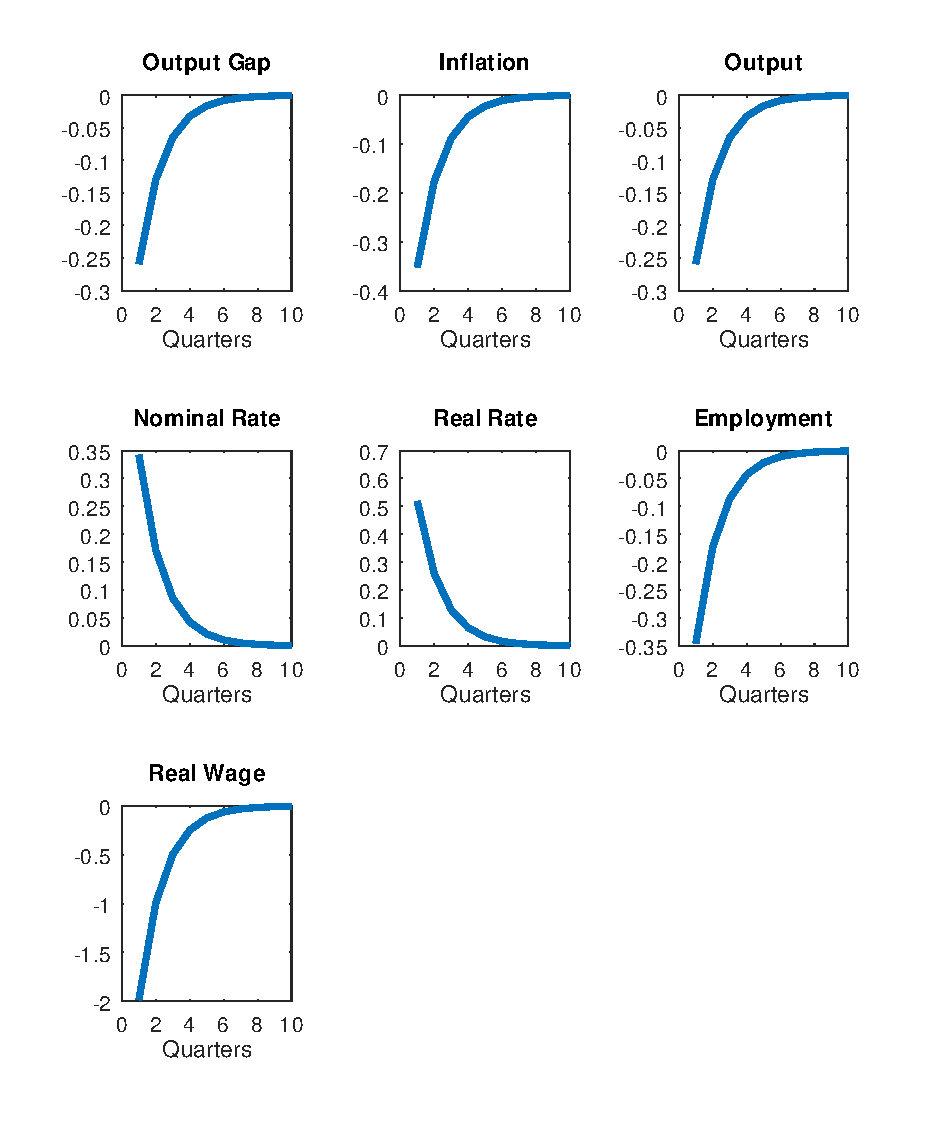
\includegraphics[width=0.57\textwidth]{Figures/v_mon_pol_irfs.pdf}}
%\caption{\label{fig:v_mon_pol_irfs} Impulse responses to monetary policy shock}
\end{figure}
 
\end{frame}

%-------------------------------------------------------

%-------------------------------------------------------
	
\begin{frame}{Impulse responses - Monetary policy shock}

\begin{itemize}
\item	The (persistent) increase in $r_{t}$ due to $i_{t} \uparrow$ (and $\pi_{t} \downarrow$) deters current expenditure
\item	Demand for final goods is reduced, and thus output and employment
\item	Recall that $y^{n}_{t}$ does not depend on $v_{t}$ so output gap declines too
\item	Reflecting this reduction in scale (and in marginal cost), firms who can initially reset prices set them lower, which underpins the initial $\pi_{t}\downarrow$ as $P_{t}\downarrow$
\item	Reduced labor demand puts downward pressure on real wage (and thus marginal cost) and this lower wage is consistent with household optimality since $-U_{n,t}/U_{c,t}$ declines due to the lower $C_{t}$ and $N_{t}$ that results from the shock
\item	Note that since $P_{t}\downarrow$ the real wage decline means $W_{t}$ must also $\downarrow \downarrow$
\item	Lower wage income also contributes to lower consumption demand
\end{itemize}

\end{frame}

%%-------------------------------------------------------
%
%%-------------------------------------------------------
%	
%\begin{frame}{Impulse responses - Time preference shock}
%
%Set $\delta_{z}$ to induce a $25$bp decline in $r^{n}_{t}$
%\begin{itemize}
%\item	Implies $z_{t}\downarrow$ on impact - as if households become more `patient'
%\item	Recall: In SDF, $Z_{t+1}/Z_{t}$ enters like $\beta$
%\item	Like a contractionary `demand' shock - but here not induced by policy
%\end{itemize}
%\begin{table}
%\begin{tabular}{ c | c }
%\textbf{Variable} 	& \textbf{Impact Effect}	\\ \hline \hline
%  Output Gap			& $-$				\\
%  Output				& $-$				\\
%  Employment		& $-$				\\
%  Real Wage			& $-$				\\
%  Real Rate			& $-$				\\
%  Nominal Rate		& $-$				\\
%  Inflation			& $-$				\\ \hline \hline
%\end{tabular}
%\end{table}
%
%Similar effects as policy shock - except in the interest rate variables
%\begin{itemize}
%\item	Can set $\delta_{z}$ to replicate effects on non-interest rate variables \emph{exactly}
%\end{itemize}
%
%\end{frame}

%-------------------------------------------------------

%-------------------------------------------------------
	
\begin{frame}{Impulse responses - Time preference shock}

Set $\delta_{z}$ to induce a $25$bp decline in $r^{n}_{t}$
\begin{itemize}
\item	Implies $z_{t}\downarrow$ on impact - as if households become more `patient'
\item	Recall: In SDF $Z_{t+1}/Z_{t}$ enters like $\beta$
\item	Like a contractionary `demand' shock - but here not induced by policy
\end{itemize}
\begin{table}
\begin{tabular}{ c | c }
\textbf{Variable} 	& \textbf{Impact Effect}	\\ \hline \hline
  Output Gap			& $-$				\\
  Output				& $-$				\\
  Employment		& $-$				\\
  Real Wage			& $-$				\\
 \textcolor{red}{Real Rate}			& \textcolor{red}{$-$}				\\
  \textcolor{red}{Nominal Rate}		& \textcolor{red}{$-$}				\\
  Inflation			& $-$				\\ \hline \hline
\end{tabular}
\end{table}

Similar effects as policy shock - \textcolor{red}{except in the interest rate variables}
\begin{itemize}
\item	Can set $\delta_{z}$ to replicate effects on non-interest rate variables \emph{exactly}
\end{itemize}

\end{frame}

%-------------------------------------------------------

%-------------------------------------------------------

\begin{frame}{Impulse responses - Time preference shock}

\begin{figure}[!htb]
\center{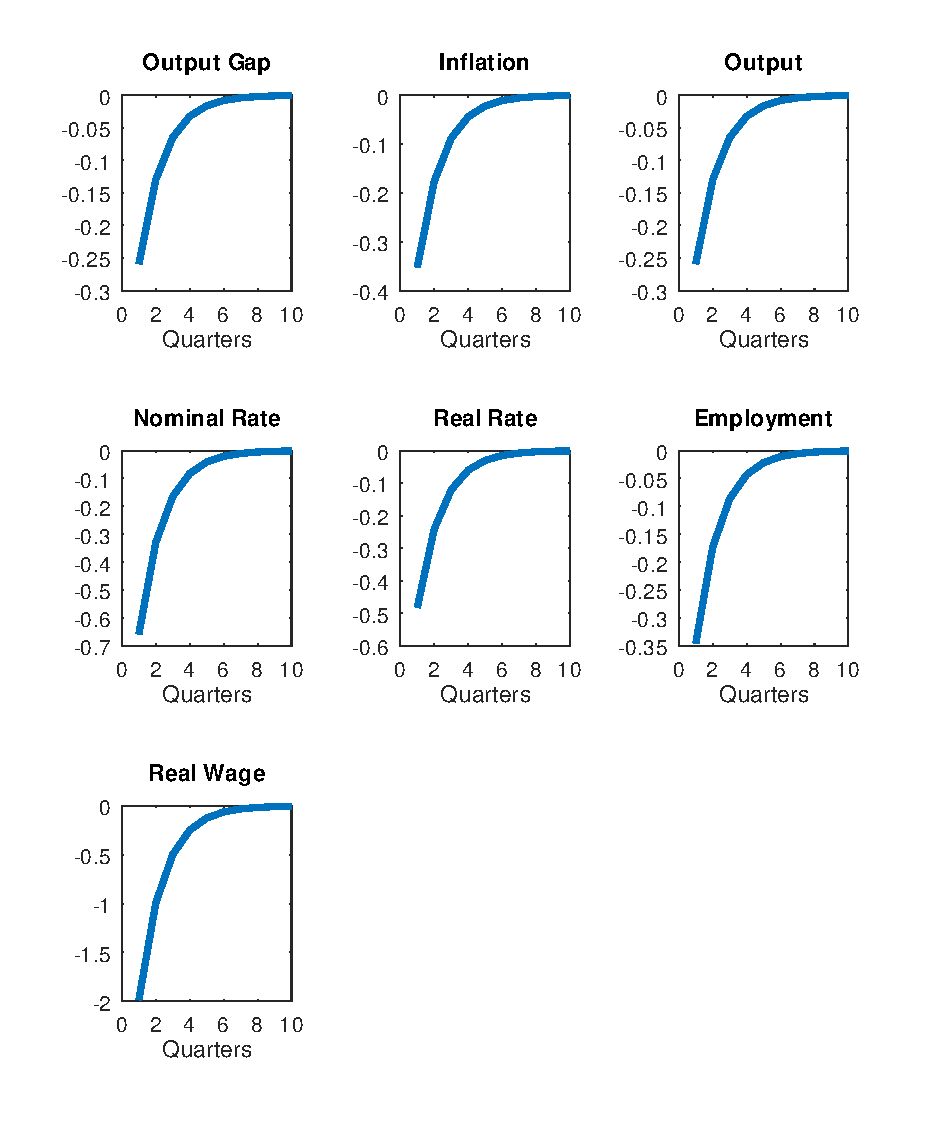
\includegraphics[width=0.57\textwidth]{Figures/z_pref_irfs.pdf}}
%\caption{\label{fig:z_pref_irfs} Impulse responses to monetary policy shock}
\end{figure}
 
\end{frame}

%-------------------------------------------------------

%-------------------------------------------------------
	
\begin{frame}{Impulse responses - Time preference shock}

Why do policy and preference shocks have (after appropriate scaling) the `same effect' on economy?
\begin{itemize}
\item	Intuitive connection between extra patience induced by preferences $\approx$ extra patience induced by prices - both act through the Euler equation
\item	Recall definition of $u_{t}$
\[
u_{t} = -\psi_{yn,a}\left( \phi_{y} + \sigma(1-\rho_{a}) \right)a_{t} + (1-\rho_{z})z_{t} - v_{t}
\]

\item	Can scale shocks to have same impact on $u_{t}$ and thus $\pi_{t}$ and $\tilde{y}_{t}$
	\begin{itemize}
	\item	If $\rho_{v} \neq \rho_{z}$ then slightly more complicated but still the same message
	\end{itemize}
\item	Why can't we say the same about $a_{t}$ (next slide)?
	\begin{itemize}
	\item	$v_{t}$ and $z_{t}$ leave $y^{n}_{t}$ unchanged so knowing movement in $\tilde{y}_{t}(\equiv y_{t}-y^{n}_{t}$) is sufficient to know movement of $y_{t}$ (and thus $n_{t}$, $w^{r}_{t}$ etc.)
	\item	$a_{t}$ affects $y^{n}_{t}$ and this will break the equivalence (though holds for $\pi_{t}$)
	\end{itemize}
\end{itemize}

\end{frame}

%-------------------------------------------------------

%-------------------------------------------------------
	
\begin{frame}{Impulse responses - Technology shock}

Consider a positive technology shock ($\delta_{a} > 0$)
\begin{table}
\begin{tabular}{ c | c}
\textbf{Variable} 	& \textbf{Impact Effect}	\\ \hline \hline
  Output Gap			& $-$				\\
  Output				& $+$				\\
  Employment		& $-$				\\
  Real Wage			& $-$				\\
  Real Rate			& $-$				\\
  Nominal Rate		& $-$				\\
  Inflation			& $-$				\\ \hline \hline
\end{tabular}
\end{table}
%\begin{table}
%\begin{tabular}{ c | c | c}
%\textbf{Variable} 	& \textbf{Impact Effect}	& \textbf{Ambiguous?}\\ \hline \hline
%  Output Gap			& $-$				&	No			\\
%  Output				& $+$				&	No			\\
%  Employment		& $-$				&	Yes			\\
%  Real Wage			& $-$				&	?			\\
%  Real Rate			& $-$				&	?			\\
%  Nominal Rate		& $-$				&	?			\\
%  Inflation			& $-$				&	?			\\ \hline \hline
%\end{tabular}
%\end{table}

Note that some of these signs depend on our choice of parameterization
\begin{itemize}
\item	$\sigma\geq1$ and $\psi_{y}$ sufficiently large $\Rightarrow$ a positive shock induces $n_{t}\downarrow$
\item	Accords with empirical evidence on effects of technology shocks
\end{itemize}

How can we reconcile this with procyclicality of $n_{t}$ in data?
\begin{itemize}
\item	Suggests shocks \emph{other than technology} may be driving business cycle
\end{itemize}

\end{frame}

%-------------------------------------------------------

%-------------------------------------------------------

\begin{frame}{Impulse responses - Technology shock}

\begin{figure}[!htb]
\center{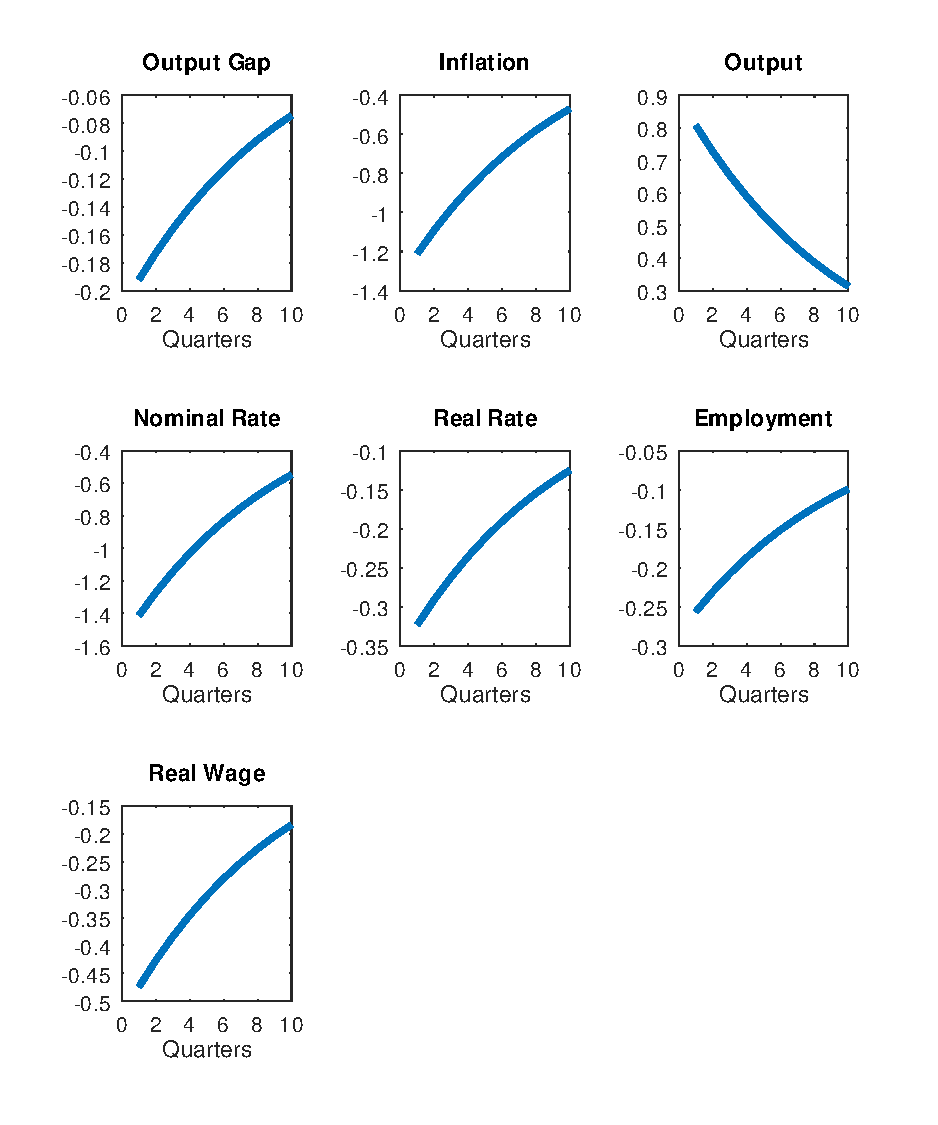
\includegraphics[width=0.57\textwidth]{Figures/a_tech_irfs.pdf}}
%\caption{\label{fig:a_tech_irfs} Impulse responses to monetary policy shock}
\end{figure}
 
\end{frame}

%-------------------------------------------------------
\section{Summary}
%-------------------------------------------------------

\begin{frame}

\begin{center}
{\LARGE Summary}
\end{center}

\end{frame}

%-------------------------------------------------------

%-------------------------------------------------------

\begin{frame}{Summary}

\begin{itemize}
\item	We have described and discussed the implications of a basic New Keynesian model
	\begin{itemize}
	\item	Specified the primitives (firm and household problems and a policy rule)
	\item	Solved for equilibrium
	\item	Analyzed the effects of shocks (under a particular parameterization)
	\end{itemize}
\vspace{3mm}	
\item	Although the model is extremely simple\ldots
	\begin{itemize}
	\item	Qualitatively, the effects of shocks are consistent with much empirical evidence
	\item	The model implies an important impact of nominal rigidities and monetary policy
	\end{itemize}
\end{itemize}
%\vspace{3mm}
%\item	We will (next set of slides) explore further the role of monetary policy
%	\begin{itemize}
%	\item	Clarifying the tradeoffs faced by policymakers
%	\item	Exploring what optimal policy should involve
%	\end{itemize}
%\end{itemize}

\end{frame}

%-------------------------------------------------------
\section{Extra Slides}
%-------------------------------------------------------

\begin{frame}

\begin{center}
{\LARGE Extra Slides}
\end{center}

\end{frame}

%-------------------------------------------------------

%-------------------------------------------------------
	
\begin{frame}[label=jump]{Equilibrium - Non-policy bloc}

Goods-level market clearing
\[
Y_{t}(i)=C_{t}(i)
\]

Given the definition of $C_{t}$ (recall equation (\ref{eqn:ds_aggregator})) it is useful to \emph{define} `aggregate output' as
\[
Y_{t} \equiv \left( \int_{0}^{1} Y_{t}\left( i \right)^{\frac{\varepsilon-1}{\varepsilon}} di \right)^{\frac{\varepsilon}{\varepsilon-1}} 
\]

Thus, we can connect $C_{t}$ in the Euler equation to the outputs of the various goods $i$, yielding
\begin{eqnarray*}
y_{t} &=& E_{t}[y_{t+1}] - \frac{1}{\sigma}\left( i_{t} - E_{t}[ \pi_{t+1} ] -  \zeta\left(z_{t}\right) \right)  \\
\zeta\left(z_{t}\right) &\equiv& \rho + \left( 1 - \rho_{z} \right) z_{t} 
\end{eqnarray*}

\end{frame}


%-------------------------------------------------------

%-------------------------------------------------------
	
\begin{frame}{Equilibrium - Non-policy bloc}

Aggregate labor demand can be obtained by aggregating over all the firms' individual labor demands (and using $C_{t}=Y_{t}$)
\[
N^{D}_{t} \equiv \int\limits_{0}^{1} N^{D}_{t}(i) di = \int\limits_{0}^{1} \left( \frac{Y_{t}(i)}{A_{t}} \right)^{\frac{1}{1-\alpha}} di = \left( \frac{Y_{t}}{A_{t}} \right)^{\frac{1}{1-\alpha}} \int\limits_{0}^{1} \left( \frac{P_{t}(i)}{P_{t}} \right)^{-\frac{\varepsilon}{1-\alpha}}di
\]

We again will be seeking log-linearity so, taking logs and rearranging
\[
n_{t}^{D} = \frac{1}{1-\alpha}(y_{t} - a_{t})
\]
where we also use
\[
d_{t}\equiv (1-\alpha)\log{\left(  \int\limits_{0}^{1} \left( \frac{P_{t}(i)}{P_{t}} \right)^{-\frac{\varepsilon}{1-\alpha}}di \right)} \stackrel{FO}{\approx} 0
\]

\end{frame}

%-------------------------------------------------------

%-------------------------------------------------------
	
\begin{frame}{Equilibrium - Non-policy bloc}

Aggregate labor demand can be obtained by aggregating over all the firms' individual labor demands (and using $C_{t}=Y_{t}$)
\[
N^{\textcolor{red}{D}}_{t} \equiv \int\limits_{0}^{1} N^{\textcolor{red}{D}}_{t}(i) di = \int\limits_{0}^{1} \left( \frac{Y_{t}(i)}{A_{t}} \right)^{\frac{1}{1-\alpha}} di = \left( \frac{Y_{t}}{A_{t}} \right)^{\frac{1}{1-\alpha}} \int\limits_{0}^{1} \left( \frac{P_{t}(i)}{P_{t}} \right)^{-\frac{\varepsilon}{1-\alpha}}di
\]

We again will be seeking log-linearity so, taking logs and rearranging
\[
n_{t}^{\textcolor{red}{D}} = \frac{1}{1-\alpha}(y_{t} - a_{t})
\]
where we also use
\[
d_{t}\equiv (1-\alpha)\log{\left(  \int\limits_{0}^{1} \left( \frac{P_{t}(i)}{P_{t}} \right)^{-\frac{\varepsilon}{1-\alpha}}di \right)} \stackrel{FO}{\approx} 0
\]

\end{frame}

%-------------------------------------------------------

%-------------------------------------------------------
	
\begin{frame}{Equilibrium - Non-policy bloc}

Aggregate labor demand can be obtained by aggregating over all the firms' individual labor demands (and using $C_{t}=Y_{t}$)
\[
N_{t} \equiv \int\limits_{0}^{1} N_{t}(i) di = \int\limits_{0}^{1} \left( \frac{Y_{t}(i)}{A_{t}} \right)^{\frac{1}{1-\alpha}} di = \left( \frac{Y_{t}}{A_{t}} \right)^{\frac{1}{1-\alpha}} \int\limits_{0}^{1} \left( \frac{P_{t}(i)}{P_{t}} \right)^{-\frac{\varepsilon}{1-\alpha}}di
\]

We again will be seeking log-linearity so, taking logs and rearranging
\[
n_{t} = \frac{1}{1-\alpha}(y_{t} - a_{t})
\]
where we also use
\[
d_{t}\equiv (1-\alpha)\log{\left(  \int\limits_{0}^{1} \left( \frac{P_{t}(i)}{P_{t}} \right)^{-\frac{\varepsilon}{1-\alpha}}di \right)} \stackrel{FO}{\approx} 0
\]

\hyperlink{jumpback}{\beamergotobutton{Back}}

\end{frame}


\end{document}
